% Created 2025-05-20 Tue 13:14
% Intended LaTeX compiler: pdflatex
\documentclass{article}


%%%%%%%% ICML 2025 EXAMPLE LATEX SUBMISSION FILE %%%%%%%%%%%%%%%%%
\usepackage[T1]{fontenc}
% Recommended, but optional, packages for figures and better typesetting:
\usepackage{microtype}
\usepackage{graphicx}
\usepackage{subfigure}
\usepackage{booktabs} % for professional tables

% hyperref makes hyperlinks in the resulting PDF.
% If your build breaks (sometimes temporarily if a hyperlink spans a page)
% please comment out the following usepackage line and replace
% \usepackage{icml2025} with \usepackage[nohyperref]{icml2025} above.
\usepackage{hyperref}


% Attempt to make hyperref and algorithmic work together better:
\newcommand{\theHalgorithm}{\arabic{algorithm}}

% Use the following line for the initial blind version submitted for review:
\usepackage[accepted]{style/icml2025}

% If accepted, instead use the following line for the camera-ready submission:
%% \usepackage[accepted]{style/icml2025}

% For theorems and such
\usepackage{amsmath}
\usepackage{amssymb}
\usepackage{mathtools}
\usepackage{amsthm}


% if you use cleveref..
\usepackage[capitalize,noabbrev]{cleveref}
%%%%%%%%%%%%%%%%%%%%%%%%%%%%%%%%
% THEOREMS
%%%%%%%%%%%%%%%%%%%%%%%%%%%%%%%%
\theoremstyle{plain}
\newtheorem{theorem}{Theorem}[section]
\newtheorem{proposition}[theorem]{Proposition}
\newtheorem{lemma}[theorem]{Lemma}
\newtheorem{corollary}[theorem]{Corollary}
\theoremstyle{definition}
\newtheorem{definition}[theorem]{Definition}
\newtheorem{assumption}[theorem]{Assumption}
\theoremstyle{remark}
\newtheorem{remark}[theorem]{Remark}

% Todonotes is useful during development; simply uncomment the next line
%    and comment out the line below the next line to turn off comments
%\usepackage[disable,textsize=tiny]{todonotes}
\usepackage[textsize=tiny]{todonotes}

% The \icmltitle you define below is probably too long as a header.
% Therefore, a short form for the running title is supplied here:
\icmltitlerunning{Test short title ICML 2025}


\usepackage[inkscapelatex=false]{svg}
\date{}
\title{}
\hypersetup{
 pdfauthor={Alan Munoz},
 pdftitle={},
 pdfkeywords={},
 pdfsubject={},
 pdfcreator={Emacs 30.1 (Org mode 9.7.11)}, 
 pdflang={English}}
\usepackage{natbib}
\begin{document}

\twocolumn[
\icmltitle{cp\_measure: Morphological profiling for data scientists}

% It is OKAY to include author information, even for blind
% submissions: the style file will automatically remove it for you
% unless you've provided the [accepted] option to the icml2025
% package.

% List of affiliations: The first argument should be a (short)
% identifier you will use later to specify author affiliations
% Academic affiliations should list Department, University, City, Region, Country
% Industry affiliations should list Company, City, Region, Country

% You can specify symbols, otherwise they are numbered in order.
% Ideally, you should not use this facility. Affiliations will be numbered
% in order of appearance and this is the preferred way.
\icmlsetsymbol{equal}{*}

\begin{icmlauthorlist}
\icmlauthor{Al\'an F. Mu\~{n}oz}{broad}
\icmlauthor{Tim Treis}{hh,broad}
\icmlauthor{Alexandr A. Kalinin}{broad}
\icmlauthor{Shatavisha Dasgupta}{broad}
\icmlauthor{Fabian Theis}{hh}
\icmlauthor{Anne E. Carpenter}{broad}
\icmlauthor{Shantanu Singh}{broad}
\end{icmlauthorlist}

\icmlaffiliation{broad}{Broad Institute of MIT and Harvard, United States}
\icmlaffiliation{hh}{Institute of Computational biology, Helmholtz Zentrum München, Germany}

\icmlcorrespondingauthor{Al\'an F. Mu\~{n}oz}{amunozgo@broadinstitute.org}
\icmlcorrespondingauthor{Shantanu Singh}{shantanu@broadinstitute.org}

% You may provide any keywords that you
% find helpful for describing your paper; these are used to populate
% the "keywords" metadata in the PDF but will not be shown in the document
\icmlkeywords{Machine Learning, ICML}

\vskip 0.3in
]

% this must go after the closing bracket ] following \twocolumn[ ...

% This command actually creates the footnote in the first column
% listing the affiliations and the copyright notice.
% The command takes one argument, which is text to display at the start of the footnote.
% The \icmlEqualContribution command is standard text for equal contribution.
% Remove it (just {}) if you do not need this facility.

\printAffiliationsAndNotice{}  % leave blank if no need to mention equal contribution
% \printAffiliationsAndNotice{\icmlEqualContribution} % otherwise use the standard text.

\begin{abstract}
Quantifying the contents of objects in images is a core challenge in biological imaging. The current tools require significant human intervention. Here we introduce our library cp\_measure, which provides programmatic access to the most widespread metrics to convert images and objects into features. We then demonstrate that the features are consistent to the standard ones and showcase tasks for which our tool is more suitable than the alternatives. cp\_measure opens the door to community-driven development and improvement of bioimage analysis metrics and pipelines, increasing the scaling capabilities, reproducibility and accessibility for computational and data scientists.
\end{abstract}
\section{Introduction}
\label{sec:org4c9ba67}
The field of biological imaging leverages data from cell microscopy images to obtain biological insights. Modern microscopes can capture a wide range of information, such as illumination and fluorescence. When coupled with fluorescence dyes or proteins biologists are able to observe the location and distribution of cells and organelles.

The main purpose of image analysis in biology is to characterize the cell state or its components. Early on, human eyes where the sole judge on this, but a more objective, scalable and reproducible method was required. This commonly entailed identifying regions of interest and calculating metrics that represent these regions, such as intensity distributions.

Morphological profiling is a technique where we generate an array of shape and intensity features for all objects, cells or otherwise. These features are fed into statistical or machine learning methods to identify patterns. One of its biggest applications is drug discovery, where scientists leverages microscopy's low acquisition cost and high throughput \citep{sealDecadeSystematicReview2024}. Morphological profiling serves not only as validation but also as information orthogonal to other high throughput methods, such as genomic sequencing.
\subsection{The current state of bioimage analysis}
\label{sec:org8f5b33d}
The most widely used software to process biological images is CellProfiler \citep{stirlingCellProfiler4Improvements2021}. Its intended audience is experimental biologists with scant programmatic experience, for whom it has been a boon. In contrast, its usefulness greatly diminishes for computer-savvy scientists who fear no command line. For them, CellProfiler means friction in pipelines comprised of multiple tools. It caters for manually-defined workflows instead of low-customization high throughput analyses, which are becoming prevalent in the age of generalist segmentation and foundational models.

Integrating a CellProfiler pipelines with other tools is a struggle. Building plug-ins to add functionality is time and effort-consuming challenges that require an understanding of its interfaces. Treating it as a black box and using its output precludes the addition of custom-made image filters. Lastly, CellProfiler depends on many number of packages from both Python and Java, amplifying the risk of dependency conflicts. Containers mitigate this problem, but not without increased complexity and caveats. To summarize, CellProfiler is an all-or-nothing tool, whose extensibility and integration with other tools demands more time and effort than most scientists can spare.

Object featurization is not exclusive of CellProfiler. For example, scikit-image can produce some overlapping features \citep{waltScikitimageImageProcessing2014}. Tools like ScaleFex or SpaCR \citep{comoletHighlyEfficientScalable2024,einarolafssonSpaCr2025} can generate features, but they have limitations: First, their implementation is completely independent and thus cannot reproduce existing datasets, potentially impacting the biological interpretations. Moreover, a common problem is that these tools enforce a structure for the input data and require wrangling with the data before processing a single image. Some alternatives, such as ScaleFex, are designed for cloud usage first, and may neglect a significant number of cases where local compute suffices. We thus believe that there is the need for a tool aimed at generalist and high throughput problems not being solved by the current software ecosystem.
\subsection{Engineered features in the era of deep learning}
\label{sec:org9dc3dfa}
The latest deep learning models can streamline image processing. Nevertheless, their capacity to provide biological interpretation is limited \citep{moenDeepLearningCellular2019}. In some cases, engineered features can even outperform learned ones \citep{tangMorphologicalProfilingDrug2024}. Compared to engineered features, deep learning approaches have a higher barrier of entry, as most models require annotating data. Foundational models, whose goal is to lower this barrier, fail to generalize well for out-of-distribution data. Unless a major change in neural networks occurs, they will still require more complex interpretability methods. Unlike learned features, whose interpretation requires complex methods like counterfactual methods or attention maps, most engineered features have a mathematical definition that is faster to calculate and easier to translate into biological concepts.

The intended audience for such a featurization tool would be, in addition to biologists, data scientists striving to achieve reproducible data analyses within a few lines of code. As a whole, engineered features still have the role of, at the minimum, complementing deep learning ones. The bioimage software ecosystems lacks a modular tool to convert images into interpretable features with no compulsory graphical interfaces or cloud compute. Ideally it should also harmonize with other scientific libraries. With all this in mind we have developed cp\_measure.
\section{Extracting interpretable features}
\label{sec:org61842b5}
In our library cp\_measure we extracted the CellProfiler measurements, removed anything that is not essential to solve the image-to-features problem and categorized the measurenents based on their input: One object and one imaging channel (e.g., intensity, texture), one object and multiple channels (e.g., Pearson correlation) and multiple objects (e.g., number of neighbours).

\begin{figure}[htbp]
\centering
\includesvg[width=.9\linewidth]{./figs/cpmeasure_overview}
\caption{\label{fig:overview}cp\_measure generates features from images by using the local information in every region of interest. It is commonly used to featurize the pairwise combination of all the available channels and objects. The resultant matrices represent the entire experiment and can be studied using machine and deep learning methods.}
\end{figure}

By isolating the numerical from the graphical and orchestration components we improved reusability, testability and extensibility. We positioned it to become a stepping stone to make the morphological profiling numerical methods accessible to the data science community. Given that the numerical internals are more transparent, we reduced the amount of time and human effort required to integrate it into pipelines, while still retaining the standard features already present in numerous datasets.

We will now demonstrate the validity and capabilities of cp\_measure in cases that would normally require domain expertise and a considerable amount of time. First, we validate cp\_measure features versus CellProfiler results with a subset of the JUMP dataset \citep{chandrasekaranJUMPCellPainting2023}. Then we showcase cases in which cp\_measure is a more practical choice to process microscopy data: First 3D images of astrocytes and then spatial transcriptomics. These use-cases demonstrate its widespread suitability for different types of problems. 
\subsection{Recapitulating CellProfiler measurements}
\label{sec:org09b0cd2}

\begin{figure}[htbp]
\centering
\includesvg[width=.9\linewidth]{./figs/jump_r2_examples}
\caption{\label{fig:cp_vs_cpmeasure}cp\_measure features match their CellProfiler analogs. \textbf{Left panel.} Representative examples comparing Cellprofiler feature values to cp\_measure's, generated using matching pairs of masks and images. \textbf{Right panel.} \(R^2\) value of a linear fit for each individual feature, comparing cp\_measure to CellProfiler.}
\end{figure}

We first performed the numerical validation that cp\_measure features, for a set of images and masks representative of the possible values, match the original CellProfiler features. For this we collected 300 images corresponding to 150 perturbations from the JUMP dataset, selecting the most significant phenotypes for a given measurement each. To ensure that we are using identical object masks, we segmented these images to obtain the cells and nuclei using CellProfiler, providing object masks and their associated features. Next, we applied cp\_measure on these masks with the original images and mapped the features from cp\_measure to CellProfiler. Lastly, we calculated a linear fit for the matched features and calculated their \(R^2\) value, indicating how well it fits a linear slope.

The initial validation of our cp\_measure features is shown on Figure \ref{fig:cp_vs_cpmeasure}. The left panel shows examples of the comparison of our features against CellProfiler's. The straight lines demonstrate the recapitulation of measurements from our implementation. A few data points fall outside the diagonals, which hint at some edge-cases are treated differently by either tool. The panel on the right shows the \(R^2\) value of a linear interpolation. Given that this value is directly correlated to the correctness of the implementation, we can see that most of our measurements have a linear relationship, regardless of whether the masks were for nuclei or cytosols. This result provides evidence that cp\_measure can be confidently in cases where CellProfiler would be used, and the insights are unlikely to change.
\subsection{Results}
\label{sec:orge5b5c6b}
\subsubsection{Astrocytes 3D data}
\label{sec:org447090b}

As a demonstration of its ease of use and the value of interpretable features, we used cp\_measure in a standard classification workflow. We processed 433 3D images of astrocytes containing 831 cells \citep{kalinin3DCellNuclear2018}. We preprocessed the data following standard procedures \citep{caicedoDataanalysisStrategiesImagebased2017}. Then, we trained a Gradient Boosting classifier to identify the day in which the image of any given cell was acquired. With this we identified which features distinguish cells on the later samples and distinguish subpopulations. Finally, we calculated the Shapley values to get a better understanding of the effects of the drugs on the cells \citep{sundararajanManyShapleyValues2020}.

\begin{figure}[htbp]
\centering
\includesvg[width=.9\linewidth]{./figs/example_shap}
\caption{\label{fig:astrocytes}\textbf{Top panel.} Example pair of astroctyes image and masks. The 3D images were projected over the z-axis, taking the maximum value across the z-stack. \textbf{Bottom panel.} Shapley values of the most important features to classify the day in which an image was taken (out of three). The test data accuracy is shown in bold.}
\end{figure}

Figure \ref{fig:astrocytes} shows an example image and object masks alongside the Shapley values of a classifier trained on our features. This indicates that the major axis length of the cell to is an indicator of phenotypic effect over the course of the experiment, implying that cells became more elongated on their minor axis. Though unsurprising, as we expect astrocytes to extend over time, cp\_measure was able to recover this with only a few lines of code.
\subsubsection{Spatial transcriptomics}
\label{sec:org5711d86}
A key advantage of providing these measurements as a standalone Python package is their ease of integration into diverse analytical workflows, which otherwise would require substantial adaptation to the standard CellProfiler environment. The recent proliferation of black-box foundation models trained solely on morphological data highlights morphology as a highly informative and predictive modality. However, the feature vectors produced by these models are typically not interpretable, preventing direct biological assessment. In contrast, classical morphological measurements yield explicit, interpretable readouts -- for instance, the co-localization of fluorescent markers -- facilitating clear biological interpretations.

To demonstrate this utility, we integrated our cp\_measure-based feature extraction into the widely used spatial analysis library Squidpy \citep{pallaSquidpyScalableFramework2022}. Being standalone allowed seamless incorporation into workflows powered by the robust SpatialData \citep{marconatoSpatialDataOpenUniversal2025} framework underlying Squidpy. Because spatial datasets often comprise significantly more cells per field-of-view (FOV) than conventional microscopy screenings -- up to approximately 100,000 cells-traditional software typically cannot process these large images without cropping, which introduces boundary artefacts. Leveraging the modular design of cp\_measure, we parallelized feature extraction at the single-cell level, streaming batches of cells across computational cores. This approach enables efficient computation even on large-scale datasets, a feat not achievable with standard CellProfiler software.

To further illustrate the value of morphological features, we evaluated their impact on cell-type prediction tasks using spatial transcriptomics data. This application is particularly compelling, as current spatial transcriptomics technologies typically produce matched histological images that remain largely underutilized beyond visualization. We analysed two mouse brain datasets generated by Bruker Spatial's CosMx platform \citep{CosMxSMIMouse2025}. Each dataset comprises expression profiles for 960 genes and immunofluorescence images captured via five distinct fluorescent probes ('Histone', 'DNA', 'GFAP', 'G', 'rRNA'). Morphological features were extracted from these 5-channel images for both datasets. Subsequently, both gene expression and morphological data were preprocessed according to best practices established by Scanpy \citep{wolfSCANPYLargescaleSinglecell2018} and Pycytominer \citep{serranoReproducibleImagebasedProfiling2025} respectively. We trained an XGBoost model to predict cell types on the larger dataset (48,556 cells; see Fig. XXX, panel XXX), comparing models using either gene expression alone or combined gene expression and morphological data. Model performance was assessed by predicting cell types in a smaller independent dataset (38,996 cells), using the F1-score metric stratified by cell type. Figure XXX (panel XXX) highlights the improved predictive accuracy obtained when morphological features are included. Importantly, this performance enhancement required no additional experimental effort, underscoring the benefit of employing cp\_measure beyond its traditional scope.

\begin{figure}[htbp]
\centering
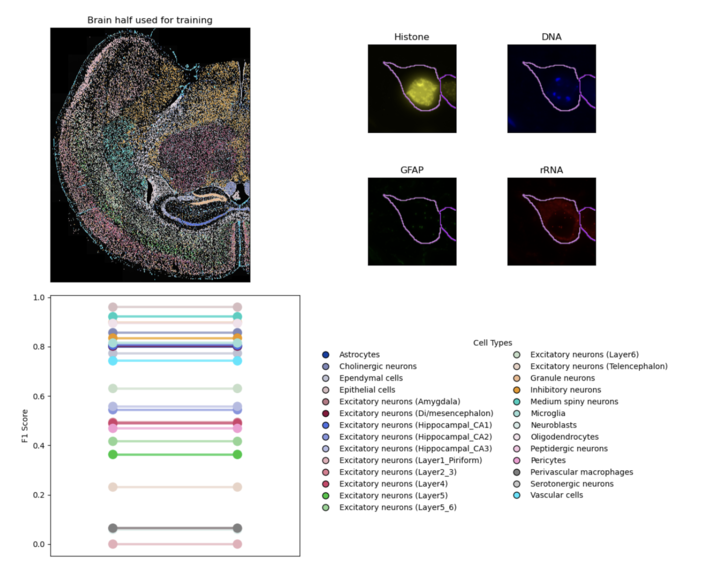
\includegraphics[width=.9\linewidth]{./figs/spatial.png}
\caption{\label{fig:spatial_omics}{[}PLACEHOLDER] Spatial omics analysis.}
\end{figure}
\section{Discussion}
\label{sec:orgf37b369}
The usage of image analysis pipelines that require manual setups hinders reproducibility and hinders our ability to compare different datasets. In this work we introduced our new library cp\_measure, which provides widely used engineered features and enables simpler automated analyses of microscopy data in either short scripts and complex pipelines. This also removes the requirement of using graphical interfaces to process microscopy data, resulting in better scaling capabilities for high-content microscopy even without cloud infrastructure.

The biologically interpretable features provided by cp\_measure complement deep learning ones and offer a better mechanistic understanding of the underlying biology. When used in tandem with generalist tools it enables more insightful pipelines that leverage machine and deep learning approaches. 

These measurements have already been used in non-biological contexts, such as environmental monitoring \citep{ideharaExploringNileRed2025}, thus these engineered metrics also benefit other scientific fields beyond morphological profiling.
\section{Future work}
\label{sec:org5cdbb12}
The most obvious way to make cp\_measure more useful is to contribute it back to CellProfiler. This would ensure that the results from pipelines built with either tool will always be comparable, while also providing the opportunity of formalizing the inputs and outputs of all measurements. 

Developing a comprehensive tests suite will guarantee mathematical correctness, which currently not even CellProfiler has. This test suite in turn would in turn expedite improvements in multiple ways: Firstly, optimizing the most compute-consuming features, such as granularity. Later on, we could add to support just-in-time compiling and GPUs.

Long-term, we envision cp\_measure can be the place to develop and distribute new measurements. While CellProfiler's measurements are already ubiquitous in bioimaging studies, the existing palette of measurements could be further extended to cover unexplored use-cases. We also see adding community-contributed measurements to better match the current questions scientists pose to imaging data.


\bibliographystyle{icml2025}
\bibliography{bibliography}
\section{Appendix}
\label{sec:orgdd18dd8}
\subsection{Methods}
\label{sec:orgb3e9382}
\subsubsection{Data and software}
\label{sec:orgbda0ae2}
The code for cp\_measure is available on \url{https://anonymous.4open.science/r/cp\_measure-B0DA}. All code to reproduce the analyses and figures, alongside links to the original data, is available on the GitHub repository \url{https://github.com/afermg/2025\_cpmeasure/}. The datasets we produced for this work are available on Zenodo, and the latest version can be found on \url{https://zenodo.org/records/15390631/latest}.
\end{document}
